\section{Preventivo} \label{section:preventivo}
Ogni componente del gruppo può ricoprire più ruoli, sia contemporaneamente che in distinti periodi del progetto, purché sia garantita l'assenza di conflitto di interessi tra i ruoli assunti.
La suddivisione del lavoro che verrà presentata di seguito garantirà un'equa ripartizione del carico di lavoro individuale e della distribuzione dei ruoli.
\subsection{Dettaglio periodi} \label{subsection:preventivo_dettaglio_periodi}
In questa sezione vengono presentati più nel dettaglio la suddivisone del lavoro e il costo preventivato per ogni periodo di sviluppo del progetto.
Nelle tabelle verranno utilizzate delle abbreviazioni per i nomi dei ruoli, come indicato nella seguente tabella:

\begin{table}[H]
  \centering
  \renewcommand{\arraystretch}{1.8}
  \rowcolors{2}{green!100!black!40}{green!100!black!30}
  \begin{tabular}{c|c}
    \rowcolor[HTML]{125E28}
    \multicolumn{1}{c}{\color[HTML]{FFFFFF}\textbf{Ruolo}}
                   & \multicolumn{1}{c}{\color[HTML]{FFFFFF}\textbf{Abbreviazione}} \\
    \hline
    Responsabile   & Re                                                             \\
    Amministratore & Am                                                             \\
    Analista       & An                                                             \\
    Progettista    & Pt                                                             \\
    Programmatore  & Pr                                                             \\
    Verificatore   & Ve
  \end{tabular}
  \caption{Abbreviazioni dei ruoli}
\end{table}

\pagebreak
%%%%%%%%%%%%%%%%%%%%%%%%%%%%%%%%%%%%%%%%%%%%%%%%%%%%%%%%%%%%%%
\subsubsection{Analisi preliminare}
Nel periodo di Analisi preliminare, ciascun componente rivestirà i ruoli secondo la seguente suddivisione:

\begin{table}[H]
  \centering
  \renewcommand{\arraystretch}{1.8}
  \rowcolors{2}{green!100!black!40}{green!100!black!30}
  \begin{tabular}{c|c|c|c|c|c|c|c}
    \rowcolor[HTML]{125E28}
    \multicolumn{1}{c}{\color[HTML]{FFFFFF}\textbf{ Nominativo }}
                         & \multicolumn{1}{c}{\color[HTML]{FFFFFF}\textbf{ Re }}
                         & \multicolumn{1}{c}{\color[HTML]{FFFFFF}\textbf{ Am}}
                         & \multicolumn{1}{c}{\color[HTML]{FFFFFF}\textbf{ An }}
                         & \multicolumn{1}{c}{\color[HTML]{FFFFFF}\textbf{ Pt }}
                         & \multicolumn{1}{c}{\color[HTML]{FFFFFF}\textbf{ Pr }}
                         & \multicolumn{1}{c}{\color[HTML]{FFFFFF}\textbf{ Ve }}
                         & \multicolumn{1}{c}{\color[HTML]{FFFFFF}\textbf{ Ore totali }}                                                                                    \\
    \hline
    Bugno Francesco      & 11                                                            & -           & 9           & -          & -          & 11          & 31           \\
    Busacca Luca         & -                                                             & 17          & 5           & -          & -          & 9           & 31           \\
    Carturan Luca        & 12                                                            & 5           & 5           & -          & -          & 9           & 31           \\
    Filosofo Michele     & -                                                             & 5           & 15          & -          & -          & 11          & 31           \\
    Furlan Dario         & -                                                             & -           & 19          & -          & -          & 12          & 31           \\
    Mattarello Francesco & -                                                             & 15          & 6           & -          & -          & 10          & 31           \\
    Midena Matteo        & -                                                             & -           & 23          & -          & -          & 9           & 32           \\
    \textbf{Ore totali}  & \textbf{23}                                                   & \textbf{42} & \textbf{82} & \textbf{-} & \textbf{-} & \textbf{71} & \textbf{218}
  \end{tabular}
  \caption{Distribuzione delle ore nel periodo di Analisi preliminare}
\end{table}

I valori sono riassunti graficamente nel seguente grafico:

\begin{figure}[H]
  \centering
  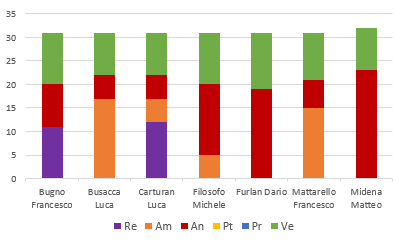
\includegraphics[scale=1.2]{immagini/ore_lavoro_analisi.png}
  \caption{Suddivisione delle ore di lavoro - Analisi preliminare}
\end{figure}

\pagebreak
%%%%%%%%%%%%%%%%%%%%%%%%%%%%%%%%%%%%%%%%%%%%%%%%%%%%%%%%%%%%%%
In questo periodo i costi da affrontare per ogni ruolo sono i seguenti:

\begin{table}[H]
  \centering
  \renewcommand{\arraystretch}{1.8}
  \rowcolors{2}{green!100!black!40}{green!100!black!30}
  \begin{tabular}{c|c|c}
    \rowcolor[HTML]{125E28}
    \multicolumn{1}{c}{\color[HTML]{FFFFFF}\textbf{Ruolo}}
                    & \multicolumn{1}{c}{\color[HTML]{FFFFFF}\textbf{Ore}}
                    & \multicolumn{1}{c}{\color[HTML]{FFFFFF}\textbf{Costo (€)}}                    \\
    \hline
    Responsabile    & 23                                                         & 690,00           \\
    Amministratore  & 42                                                         & 840,00           \\
    Analista        & 82                                                         & 2050,00          \\
    Progettista     & -                                                          & -                \\
    Programmatore   & -                                                          & -                \\
    Verificatore    & 71                                                         & 1065,00          \\
    \textbf{Totale} & \textbf{218}                                               & \textbf{4645,00}
  \end{tabular}
  \caption{Prospetto dei costi per ruolo nel periodo di Analisi preliminare}
\end{table}

\begin{figure}[H]
  \centering
  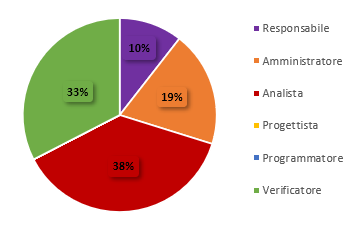
\includegraphics[scale=1]{immagini/ore_ruolo_analisi.png}
  \caption{Ore per ruolo sul totale - Analisi preliminare}
\end{figure}

\begin{figure}[H]
  \centering
  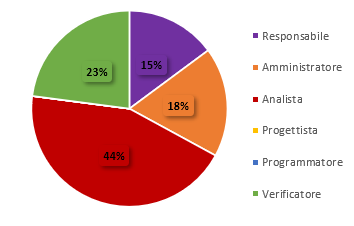
\includegraphics[scale=1]{immagini/costo_ruolo_analisi.png}
  \caption{Costo per ruolo sul totale - Analisi preliminare}
\end{figure}

%%%%%%%%%%%%%%%%%%%%%%%%%%%%%%%%%%%%%%%%%%%%%%%%%%%%%%%%%%%%%%

\subsubsection{Progettazione Technology Baseline}
Nel periodo di Progettazione per la Technology Baseline, ciascun componente rivestirà i ruoli secondo la seguente suddivisione:

\begin{table}[H]
  \centering
  \renewcommand{\arraystretch}{1.8}
  \rowcolors{2}{green!100!black!40}{green!100!black!30}
  \begin{tabular}{c|c|c|c|c|c|c|c}
    \rowcolor[HTML]{125E28}
    \multicolumn{1}{c}{\color[HTML]{FFFFFF}\textbf{ Nominativo }}
                         & \multicolumn{1}{c}{\color[HTML]{FFFFFF}\textbf{ Re }}
                         & \multicolumn{1}{c}{\color[HTML]{FFFFFF}\textbf{ Am}}
                         & \multicolumn{1}{c}{\color[HTML]{FFFFFF}\textbf{ An }}
                         & \multicolumn{1}{c}{\color[HTML]{FFFFFF}\textbf{ Pt }}
                         & \multicolumn{1}{c}{\color[HTML]{FFFFFF}\textbf{ Pr }}
                         & \multicolumn{1}{c}{\color[HTML]{FFFFFF}\textbf{ Ve }}
                         & \multicolumn{1}{c}{\color[HTML]{FFFFFF}\textbf{ Ore totali }}                                                                                   \\
    \hline
    Bugno Francesco      & -                                                             & 2          & 3           & 3           & -          & 3           & 11          \\
    Busacca Luca         & -                                                             & -          & -           & 6           & -          & 4           & 10          \\
    Carturan Luca        & -                                                             & -          & 5           & 6           & -          & -           & 11          \\
    Filosofo Michele     & -                                                             & 3          & -           & 4           & -          & 4           & 11          \\
    Furlan Dario         & 7                                                             & -          & -           & 5           & -          & -           & 12          \\
    Mattarello Francesco & -                                                             & -          & 4           & 4           & -          & 3           & 11          \\
    Midena Matteo        & -                                                             & 3          & -           & 5           & -          & 3           & 11          \\
    \textbf{Ore totali}  & \textbf{7}                                                    & \textbf{8} & \textbf{12} & \textbf{33} & \textbf{-} & \textbf{17} & \textbf{77}
  \end{tabular}
  \caption{Distribuzione delle ore nel periodo di Progettazione Technology Baseline}
\end{table}

I valori sono riassunti graficamente nel seguente grafico:

\begin{figure}[H]
  \centering
  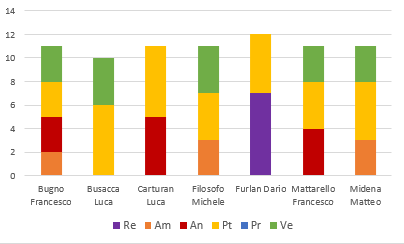
\includegraphics[scale=1.2]{immagini/ore_lavoro_TB.png}
  \caption{Suddivisione delle ore di lavoro - Progettazione Technology Baseline}
\end{figure}

\pagebreak
%%%%%%%%%%%%%%%%%%%%%%%%%%%%%%%%%%%%%%%%%%%%%%%%%%%%%%%%%%%%%%
In questo periodo i costi da affrontare per ogni ruolo sono i seguenti:

\begin{table}[H]
  \centering
  \renewcommand{\arraystretch}{1.8}
  \rowcolors{2}{green!100!black!40}{green!100!black!30}
  \begin{tabular}{c|c|c}
    \rowcolor[HTML]{125E28}
    \multicolumn{1}{c}{\color[HTML]{FFFFFF}\textbf{Ruolo}}
                    & \multicolumn{1}{c}{\color[HTML]{FFFFFF}\textbf{Ore}}
                    & \multicolumn{1}{c}{\color[HTML]{FFFFFF}\textbf{Costo (€)}}                    \\
    \hline
    Responsabile    & 7                                                          & 210,00           \\
    Amministratore  & 8                                                          & 160,00           \\
    Analista        & 12                                                         & 300,00           \\
    Progettista     & 33                                                         & 825,00           \\
    Programmatore   & -                                                          & -                \\
    Verificatore    & 17                                                         & 255,00           \\
    \textbf{Totale} & \textbf{77}                                                & \textbf{1750,00}
  \end{tabular}
  \caption{Prospetto dei costi per ruolo nel periodo di Progettazione Technology Baseline}
\end{table}

\begin{figure}[H]
  \centering
  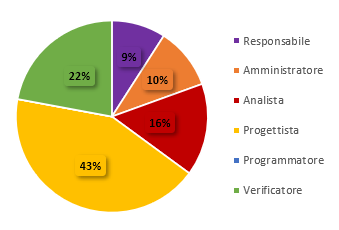
\includegraphics[scale=1]{immagini/ore_ruolo_TB.png}
  \caption{Ore per ruolo sul totale - Progettazione Technology Baseline}
\end{figure}

\begin{figure}[H]
  \centering
  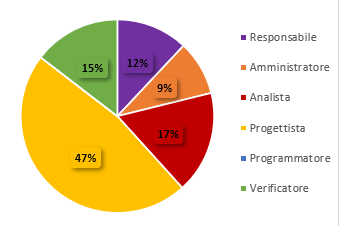
\includegraphics[scale=1]{immagini/costo_ruolo_TB.png}
  \caption{Costo per ruolo sul totale - Progettazione Technology Baseline}
\end{figure}

%%%%%%%%%%%%%%%%%%%%%%%%%%%%%%%%%%%%%%%%%%%%%%%%%%%%%%%%%%%%%%
\subsubsection{Codifica Proof of Concept}
Nel periodo di Codifica del Proof of Concept\glo{}, ciascun componente rivestirà i ruoli secondo la seguente suddivisione:

\begin{table}[H]
  \centering
  \renewcommand{\arraystretch}{1.8}
  \rowcolors{2}{green!100!black!40}{green!100!black!30}
  \begin{tabular}{c|c|c|c|c|c|c|c}
    \rowcolor[HTML]{125E28}
    \multicolumn{1}{c}{\color[HTML]{FFFFFF}\textbf{ Nominativo }}
                         & \multicolumn{1}{c}{\color[HTML]{FFFFFF}\textbf{ Re }}
                         & \multicolumn{1}{c}{\color[HTML]{FFFFFF}\textbf{ Am}}
                         & \multicolumn{1}{c}{\color[HTML]{FFFFFF}\textbf{ An }}
                         & \multicolumn{1}{c}{\color[HTML]{FFFFFF}\textbf{ Pt }}
                         & \multicolumn{1}{c}{\color[HTML]{FFFFFF}\textbf{ Pr }}
                         & \multicolumn{1}{c}{\color[HTML]{FFFFFF}\textbf{ Ve }}
                         & \multicolumn{1}{c}{\color[HTML]{FFFFFF}\textbf{ Ore totali }}                                                                                    \\
    \hline
    Bugno Francesco      & -                                                             & -          & -          & 7           & 4           & 6           & 17           \\
    Busacca Luca         & -                                                             & -          & 3          & 5           & 7           & 4           & 19           \\
    Carturan Luca        & -                                                             & -          & -          & 6           & 8           & 3           & 17           \\
    Filosofo Michele     & -                                                             & -          & 4          & 4           & 7           & 3           & 18           \\
    Furlan Dario         & -                                                             & 2          & -          & 8           & 8           & -           & 18           \\
    Mattarello Francesco & -                                                             & 3          & -          & 6           & 2           & 7           & 18           \\
    Midena Matteo        & 8                                                             & -          & -          & 2           & 8           & -           & 18           \\
    \textbf{Ore totali}  & \textbf{8}                                                    & \textbf{5} & \textbf{7} & \textbf{38} & \textbf{44} & \textbf{23} & \textbf{125}
  \end{tabular}
  \caption{Distribuzione delle ore nel periodo di Codifica Proof of Concept}
\end{table}

I valori sono riassunti graficamente nel seguente grafico:

\begin{figure}[H]
  \centering
  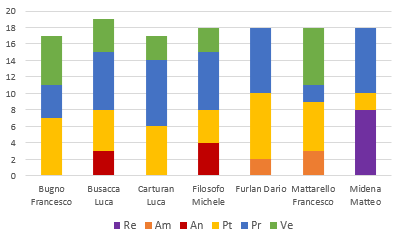
\includegraphics[scale=1.2]{immagini/ore_lavoro_PoC.png}
  \caption{Suddivisione delle ore di lavoro - Codifica Proof of Concept}
\end{figure}

\pagebreak
%%%%%%%%%%%%%%%%%%%%%%%%%%%%%%%%%%%%%%%%%%%%%%%%%%%%%%%%%%%%%%
In questo periodo i costi da affrontare per ogni ruolo sono i seguenti:

\begin{table}[H]
  \centering
  \renewcommand{\arraystretch}{1.8}
  \rowcolors{2}{green!100!black!40}{green!100!black!30}
  \begin{tabular}{c|c|c}
    \rowcolor[HTML]{125E28}
    \multicolumn{1}{c}{\color[HTML]{FFFFFF}\textbf{Ruolo}}
                    & \multicolumn{1}{c}{\color[HTML]{FFFFFF}\textbf{Ore}}
                    & \multicolumn{1}{c}{\color[HTML]{FFFFFF}\textbf{Costo (€)}}                    \\
    \hline
    Responsabile    & 8                                                          & 240,00           \\
    Amministratore  & 5                                                          & 100,00           \\
    Analista        & 7                                                          & 175,00           \\
    Progettista     & 38                                                         & 950,00           \\
    Programmatore   & 44                                                         & 660,00           \\
    Verificatore    & 23                                                         & 345,00           \\
    \textbf{Totale} & \textbf{125}                                               & \textbf{2470,00}
  \end{tabular}
  \caption{Prospetto dei costi per ruolo nel periodo di Codifica Proof of Concept}
\end{table}

\begin{figure}[H]
  \centering
  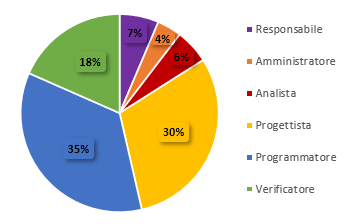
\includegraphics[scale=1]{immagini/ore_ruolo_PoC.png}
  \caption{Ore per ruolo sul totale - Codifica Proof of Concept}
\end{figure}

\begin{figure}[H]
  \centering
  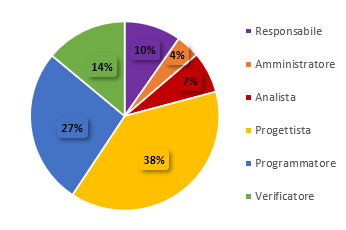
\includegraphics[scale=1]{immagini/costo_ruolo_PoC.png}
  \caption{Costo per ruolo sul totale - Codifica Proof of Concept}
\end{figure}

%%%%%%%%%%%%%%%%%%%%%%%%%%%%%%%%%%%%%%%%%%%%%%%%%%%%%%%%%%%%%%

\subsubsection{Progettazione di dettaglio e codifica dei requisiti} \label{subsubsection:preventivo_progettazione_dettaglio}
\paragraph{Sprint 1} \label{paragraph:preventivo_sprint1}
Nel primo Sprint\glo{}, ciascun componente rivestirà i ruoli secondo la seguente suddivisione:

\begin{table}[H]
  \centering
  \renewcommand{\arraystretch}{1.8}
  \rowcolors{2}{green!100!black!40}{green!100!black!30}
  \begin{tabular}{c|c|c|c|c|c|c|c}
    \rowcolor[HTML]{125E28}
    \multicolumn{1}{c}{\color[HTML]{FFFFFF}\textbf{ Nominativo }}
                         & \multicolumn{1}{c}{\color[HTML]{FFFFFF}\textbf{ Re }}
                         & \multicolumn{1}{c}{\color[HTML]{FFFFFF}\textbf{ Am}}
                         & \multicolumn{1}{c}{\color[HTML]{FFFFFF}\textbf{ An }}
                         & \multicolumn{1}{c}{\color[HTML]{FFFFFF}\textbf{ Pt }}
                         & \multicolumn{1}{c}{\color[HTML]{FFFFFF}\textbf{ Pr }}
                         & \multicolumn{1}{c}{\color[HTML]{FFFFFF}\textbf{ Ve }}
                         & \multicolumn{1}{c}{\color[HTML]{FFFFFF}\textbf{ Ore totali }}                                                                                   \\
    \hline
    Bugno Francesco      & -                                                             & -          & -          & 3           & 4           & 3           & 10          \\
    Busacca Luca         & -                                                             & -          & 3          & -           & 4           & 3           & 10          \\
    Carturan Luca        & -                                                             & -          & 1          & 3           & 4           & 3           & 11          \\
    Filosofo Michele     & 4                                                             & -          & -          & 3           & -           & 3           & 10          \\
    Furlan Dario         & -                                                             & 3          & -          & 4           & -           & 3           & 10          \\
    Mattarello Francesco & -                                                             & -          & 1          & 4           & 5           & -           & 10          \\
    Midena Matteo        & -                                                             & -          & 1          & 4           & 6           & -           & 11          \\
    \textbf{Ore totali}  & \textbf{4}                                                    & \textbf{3} & \textbf{6} & \textbf{21} & \textbf{23} & \textbf{15} & \textbf{72}
  \end{tabular}
  \caption{Distribuzione delle ore durante il primo Sprint}
\end{table}

I valori sono riassunti graficamente nel seguente grafico:

\begin{figure}[H]
  \centering
  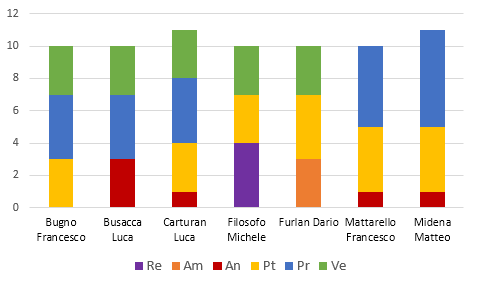
\includegraphics[scale=1.0]{immagini/1Sprint_oreLavoro.png}
  \caption{Suddivisione delle ore di lavoro - Sprint 1}
\end{figure}

\pagebreak
%%%%%%%%%%%%%%%%%%%%%%%%%%%%%%%%%%%%%%%%%%%%%%%%%%%%%%%%%%%%%%
In questo periodo i costi da affrontare per ogni ruolo sono i seguenti:

\begin{table}[H]
  \centering
  \renewcommand{\arraystretch}{1.8}
  \rowcolors{2}{green!100!black!40}{green!100!black!30}
  \begin{tabular}{c|c|c}
    \rowcolor[HTML]{125E28}
    \multicolumn{1}{c}{\color[HTML]{FFFFFF}\textbf{Ruolo}}
                    & \multicolumn{1}{c}{\color[HTML]{FFFFFF}\textbf{Ore}}
                    & \multicolumn{1}{c}{\color[HTML]{FFFFFF}\textbf{Costo (€)}}                    \\
    \hline
    Responsabile    & 4                                                          & 120,00           \\
    Amministratore  & 3                                                          & 60,00            \\
    Analista        & 6                                                          & 150,00           \\
    Progettista     & 21                                                         & 525,00           \\
    Programmatore   & 23                                                         & 345,00           \\
    Verificatore    & 15                                                         & 225,00           \\
    \textbf{Totale} & \textbf{72}                                                & \textbf{1425,00}
  \end{tabular}
  \caption{Prospetto dei costi per ruolo - Sprint 1}
\end{table}

\begin{figure}[H]
  \centering
  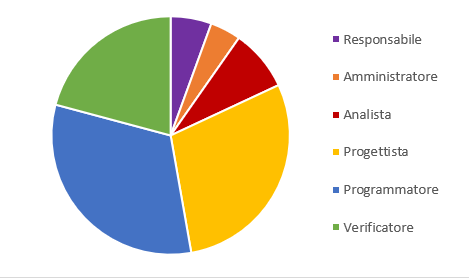
\includegraphics[scale=0.8]{immagini/1Sprint_oreRuolo.png}
  \caption{Ore per ruolo sul totale - Sprint 1}
\end{figure}

\begin{figure}[H]
  \centering
  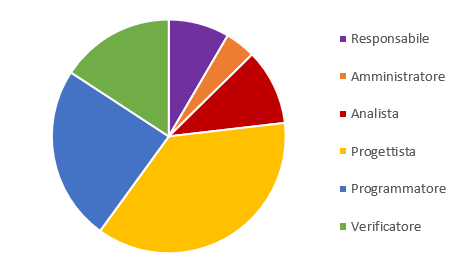
\includegraphics[scale=0.8]{immagini/1Sprint_costoRuolo.png}
  \caption{Costo per ruolo sul totale - Sprint 1}
\end{figure}
\pagebreak

%%%%%%%%%%%%%%%%%%%%%%%%%%%%%%%%%%%%%%%%%%%%%%%%%%%%%%%%%%%%%%%%%%%%%%%%%%%%%%%%%%%%%%%%%%%

\paragraph{Sprint 2} \label{paragraph:preventivo_sprint2}
Nel secondo Sprint\glo{}, ciascun componente rivestirà i ruoli secondo la seguente suddivisione:

\begin{table}[H]
  \centering
  \renewcommand{\arraystretch}{1.8}
  \rowcolors{2}{green!100!black!40}{green!100!black!30}
  \begin{tabular}{c|c|c|c|c|c|c|c}
    \rowcolor[HTML]{125E28}
    \multicolumn{1}{c}{\color[HTML]{FFFFFF}\textbf{ Nominativo }}
                         & \multicolumn{1}{c}{\color[HTML]{FFFFFF}\textbf{ Re }}
                         & \multicolumn{1}{c}{\color[HTML]{FFFFFF}\textbf{ Am}}
                         & \multicolumn{1}{c}{\color[HTML]{FFFFFF}\textbf{ An }}
                         & \multicolumn{1}{c}{\color[HTML]{FFFFFF}\textbf{ Pt }}
                         & \multicolumn{1}{c}{\color[HTML]{FFFFFF}\textbf{ Pr }}
                         & \multicolumn{1}{c}{\color[HTML]{FFFFFF}\textbf{ Ve }}
                         & \multicolumn{1}{c}{\color[HTML]{FFFFFF}\textbf{ Ore totali }}                                                                                   \\
    \hline
    Bugno Francesco      & -                                                             & -          & 1          & 4           & 5           & -           & 10          \\
    Busacca Luca         & 3                                                             & -          & -          & 3           & 2           & 2           & 10          \\
    Carturan Luca        & -                                                             & -          & -          & 2           & 4           & 3           & 9           \\
    Filosofo Michele     & -                                                             & -          & 2          & -           & 5           & 2           & 9           \\
    Furlan Dario         & -                                                             & -          & -          & 4           & 5           & 1           & 10          \\
    Mattarello Francesco & -                                                             & -          & -          & 3           & 4           & 2           & 9           \\
    Midena Matteo        & -                                                             & 4          & -          & -           & 3           & 3           & 10          \\
    \textbf{Ore totali}  & \textbf{3}                                                    & \textbf{4} & \textbf{3} & \textbf{16} & \textbf{28} & \textbf{13} & \textbf{67}
  \end{tabular}
  \caption{Distribuzione delle ore durante il secondo Sprint}
\end{table}

I valori sono riassunti graficamente nel seguente grafico:

\begin{figure}[H]
  \centering
  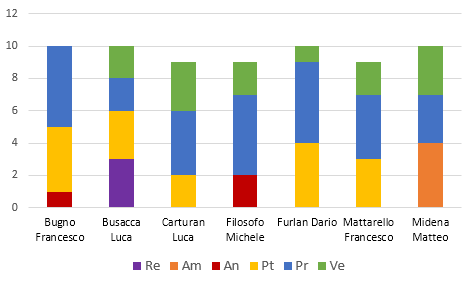
\includegraphics[scale=1.0]{immagini/2Sprint_oreLavoro.png}
  \caption{Suddivisione delle ore di lavoro - Sprint 2}
\end{figure}

\pagebreak
%%%%%%%%%%%%%%%%%%%%%%%%%%%%%%%%%%%%%%%%%%%%%%%%%%%%%%%%%%%%%%
In questo periodo i costi da affrontare per ogni ruolo sono i seguenti:

\begin{table}[H]
  \centering
  \renewcommand{\arraystretch}{1.8}
  \rowcolors{2}{green!100!black!40}{green!100!black!30}
  \begin{tabular}{c|c|c}
    \rowcolor[HTML]{125E28}
    \multicolumn{1}{c}{\color[HTML]{FFFFFF}\textbf{Ruolo}}
                    & \multicolumn{1}{c}{\color[HTML]{FFFFFF}\textbf{Ore}}
                    & \multicolumn{1}{c}{\color[HTML]{FFFFFF}\textbf{Costo (€)}}                    \\
    \hline
    Responsabile    & 3                                                          & 90,00            \\
    Amministratore  & 4                                                          & 80,00            \\
    Analista        & 3                                                          & 75,00            \\
    Progettista     & 16                                                         & 400,00           \\
    Programmatore   & 28                                                         & 420,00           \\
    Verificatore    & 13                                                         & 195,00           \\
    \textbf{Totale} & \textbf{67}                                                & \textbf{1260,00}
  \end{tabular}
  \caption{Prospetto dei costi per ruolo - Sprint 2}
\end{table}

\begin{figure}[H]
  \centering
  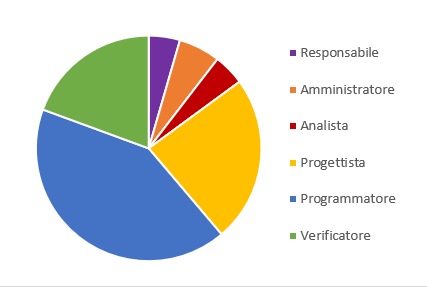
\includegraphics[scale=0.8]{immagini/2Sprint_oreRuolo.png}
  \caption{Ore per ruolo sul totale - Sprint 2}
\end{figure}

\begin{figure}[H]
  \centering
  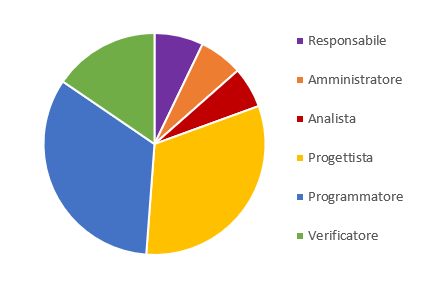
\includegraphics[scale=0.8]{immagini/2Sprint_costoRuolo.png}
  \caption{Costo per ruolo sul totale - Sprint 2}
\end{figure}
\pagebreak
%%%%%%%%%%%%%%%%%%%%%%%%%%%%%%%%%%%%%%%%%%%%%%%%%%%%%%%%%%%%%%

\paragraph{Sprint 3} \label{paragraph:preventivo_sprint3}
Nel terzo Sprint\glo{}, ciascun componente rivestirà i ruoli secondo la seguente suddivisione:

\begin{table}[H]
  \centering
  \renewcommand{\arraystretch}{1.8}
  \rowcolors{2}{green!100!black!40}{green!100!black!30}
  \begin{tabular}{c|c|c|c|c|c|c|c}
    \rowcolor[HTML]{125E28}
    \multicolumn{1}{c}{\color[HTML]{FFFFFF}\textbf{ Nominativo }}
                         & \multicolumn{1}{c}{\color[HTML]{FFFFFF}\textbf{ Re }}
                         & \multicolumn{1}{c}{\color[HTML]{FFFFFF}\textbf{ Am}}
                         & \multicolumn{1}{c}{\color[HTML]{FFFFFF}\textbf{ An }}
                         & \multicolumn{1}{c}{\color[HTML]{FFFFFF}\textbf{ Pt }}
                         & \multicolumn{1}{c}{\color[HTML]{FFFFFF}\textbf{ Pr }}
                         & \multicolumn{1}{c}{\color[HTML]{FFFFFF}\textbf{ Ve }}
                         & \multicolumn{1}{c}{\color[HTML]{FFFFFF}\textbf{ Ore totali }}                                                                                   \\
    \hline
    Bugno Francesco      & -                                                             & 2          & -          & -           & 4           & 2           & 8           \\
    Busacca Luca         & -                                                             & -          & -          & 3           & 3           & 2           & 8           \\
    Carturan Luca        & -                                                             & -          & -          & 2           & 3           & 2           & 7           \\
    Filosofo Michele     & -                                                             & -          & -          & 4           & 4           & -           & 8           \\
    Furlan Dario         & -                                                             & -          & -          & 1           & 4           & 3           & 8           \\
    Mattarello Francesco & 2                                                             & -          & -          & 3           & -           & 2           & 7           \\
    Midena Matteo        & -                                                             & -          & -          & 3           & 3           & 2           & 8           \\
    \textbf{Ore totali}  & \textbf{2}                                                    & \textbf{2} & \textbf{-} & \textbf{16} & \textbf{21} & \textbf{13} & \textbf{54}
  \end{tabular}
  \caption{Distribuzione delle ore durante il terzo Sprint}
\end{table}

I valori sono riassunti graficamente nel seguente grafico:

\begin{figure}[H]
  \centering
  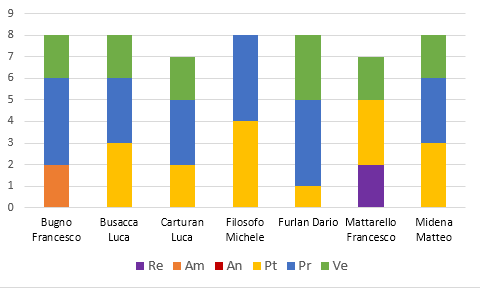
\includegraphics[scale=1.0]{immagini/3Sprint_oreLavoro.png}
  \caption{Suddivisione delle ore di lavoro - Sprint 3}
\end{figure}

\pagebreak
%%%%%%%%%%%%%%%%%%%%%%%%%%%%%%%%%%%%%%%%%%%%%%%%%%%%%%%%%%%%%%
In questo periodo i costi da affrontare per ogni ruolo sono i seguenti:

\begin{table}[H]
  \centering
  \renewcommand{\arraystretch}{1.8}
  \rowcolors{2}{green!100!black!40}{green!100!black!30}
  \begin{tabular}{c|c|c}
    \rowcolor[HTML]{125E28}
    \multicolumn{1}{c}{\color[HTML]{FFFFFF}\textbf{Ruolo}}
                    & \multicolumn{1}{c}{\color[HTML]{FFFFFF}\textbf{Ore}}
                    & \multicolumn{1}{c}{\color[HTML]{FFFFFF}\textbf{Costo (€)}}                    \\
    \hline
    Responsabile    & 2                                                          & 60,00            \\
    Amministratore  & 2                                                          & 40,00            \\
    Analista        & -                                                          & -                \\
    Progettista     & 16                                                         & 400,00           \\
    Programmatore   & 21                                                         & 315,00           \\
    Verificatore    & 13                                                         & 195,00           \\
    \textbf{Totale} & \textbf{54}                                                & \textbf{1010,00}
  \end{tabular}
  \caption{Prospetto dei costi per ruolo - Sprint 3}
\end{table}

\begin{figure}[H]
  \centering
  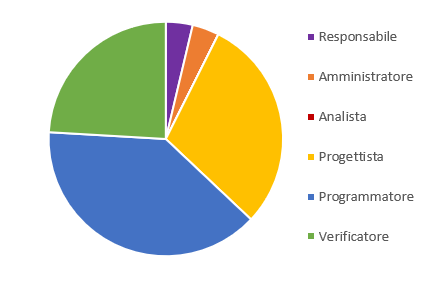
\includegraphics[scale=0.8]{immagini/3Sprint_oreRuolo.png}
  \caption{Ore per ruolo sul totale - Sprint 3}
\end{figure}

\begin{figure}[H]
  \centering
  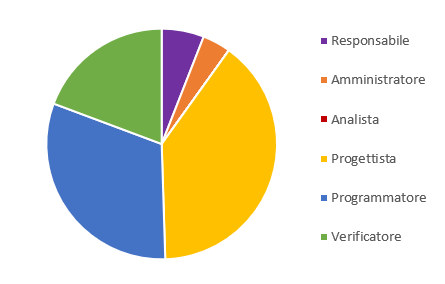
\includegraphics[scale=0.8]{immagini/3Sprint_costoRuolo.png}
  \caption{Costo per ruolo sul totale - Sprint 3}
\end{figure}
\pagebreak
%%%%%%%%%%%%%%%%%%%%%%%%%%%%%%%%%%%%%%%%%%%%%%%%%%%%%%%%%%%%%%

\paragraph{Sprint 4} \label{paragraph:preventivo_sprint4}
Nel quarto Sprint\glo{}, ciascun componente rivestirà i ruoli secondo la seguente suddivisione:

\begin{table}[H]
  \centering
  \renewcommand{\arraystretch}{1.8}
  \rowcolors{2}{green!100!black!40}{green!100!black!30}
  \begin{tabular}{c|c|c|c|c|c|c|c}
    \rowcolor[HTML]{125E28}
    \multicolumn{1}{c}{\color[HTML]{FFFFFF}\textbf{ Nominativo }}
                         & \multicolumn{1}{c}{\color[HTML]{FFFFFF}\textbf{ Re }}
                         & \multicolumn{1}{c}{\color[HTML]{FFFFFF}\textbf{ Am}}
                         & \multicolumn{1}{c}{\color[HTML]{FFFFFF}\textbf{ An }}
                         & \multicolumn{1}{c}{\color[HTML]{FFFFFF}\textbf{ Pt }}
                         & \multicolumn{1}{c}{\color[HTML]{FFFFFF}\textbf{ Pr }}
                         & \multicolumn{1}{c}{\color[HTML]{FFFFFF}\textbf{ Ve }}
                         & \multicolumn{1}{c}{\color[HTML]{FFFFFF}\textbf{ Ore totali }}                                                                                  \\
    \hline
    Bugno Francesco      & -                                                             & -          & -          & 2           & 3           & -          & 5           \\
    Busacca Luca         & -                                                             & -          & -          & 2           & 2           & 1          & 5           \\
    Carturan Luca        & 1                                                             & -          & -          & 2           & -           & 2          & 5           \\
    Filosofo Michele     & -                                                             & -          & -          & 3           & 2           & -          & 5           \\
    Furlan Dario         & -                                                             & -          & -          & 2           & 2           & 1          & 5           \\
    Mattarello Francesco & -                                                             & 1          & -          & 2           & 2           & -          & 5           \\
    Midena Matteo        & -                                                             & -          & -          & 2           & 2           & 1          & 5           \\
    \textbf{Ore totali}  & \textbf{1}                                                    & \textbf{1} & \textbf{-} & \textbf{15} & \textbf{13} & \textbf{5} & \textbf{35}
  \end{tabular}
  \caption{Distribuzione delle ore durante il quarto Sprint}
\end{table}

I valori sono riassunti graficamente nel seguente grafico:

\begin{figure}[H]
  \centering
  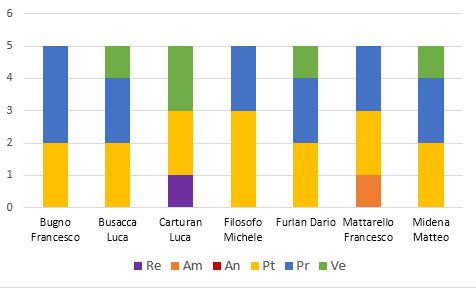
\includegraphics[scale=1.0]{immagini/4Sprint_oreLavoro.png}
  \caption{Suddivisione delle ore di lavoro - Sprint 4}
\end{figure}

\pagebreak
%%%%%%%%%%%%%%%%%%%%%%%%%%%%%%%%%%%%%%%%%%%%%%%%%%%%%%%%%%%%%%
In questo periodo i costi da affrontare per ogni ruolo sono i seguenti:

\begin{table}[H]
  \centering
  \renewcommand{\arraystretch}{1.8}
  \rowcolors{2}{green!100!black!40}{green!100!black!30}
  \begin{tabular}{c|c|c}
    \rowcolor[HTML]{125E28}
    \multicolumn{1}{c}{\color[HTML]{FFFFFF}\textbf{Ruolo}}
                    & \multicolumn{1}{c}{\color[HTML]{FFFFFF}\textbf{Ore}}
                    & \multicolumn{1}{c}{\color[HTML]{FFFFFF}\textbf{Costo (€)}}                   \\
    \hline
    Responsabile    & 1                                                          & 30,00           \\
    Amministratore  & 1                                                          & 20,00           \\
    Analista        & -                                                          & -               \\
    Progettista     & 15                                                         & 375,00          \\
    Programmatore   & 13                                                         & 195,00          \\
    Verificatore    & 5                                                          & 75,00           \\
    \textbf{Totale} & \textbf{35}                                                & \textbf{695,00}
  \end{tabular}
  \caption{Prospetto dei costi per ruolo - Sprint 4}
\end{table}

\begin{figure}[H]
  \centering
  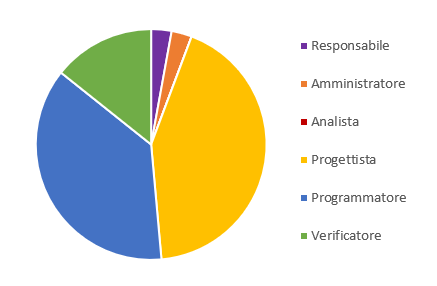
\includegraphics[scale=0.8]{immagini/4Sprint_oreRuolo.png}
  \caption{Ore per ruolo sul totale - Sprint 4}
\end{figure}

\begin{figure}[H]
  \centering
  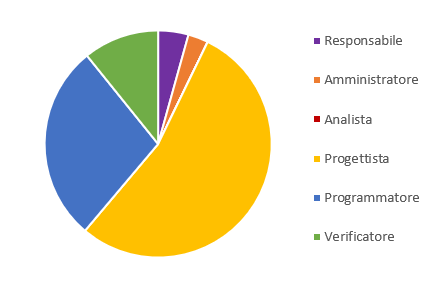
\includegraphics[scale=0.8]{immagini/4Sprint_costoRuolo.png}
  \caption{Costo per ruolo sul totale - Sprint 4}
\end{figure}
\pagebreak

%%%%%%%%%%%%%%%%%%%%%%%%%%%%%%%%%%%%%%%%%%%%%%%%%%%%%%%%%%%%%%

\paragraph{Sprint 5} \label{paragraph:preventivo_sprint5}
Nel quinto Sprint\glo{}, ciascun componente rivestirà i ruoli secondo la seguente suddivisione:

\begin{table}[H]
  \centering
  \renewcommand{\arraystretch}{1.8}
  \rowcolors{2}{green!100!black!40}{green!100!black!30}
  \begin{tabular}{c|c|c|c|c|c|c|c}
    \rowcolor[HTML]{125E28}
    \multicolumn{1}{c}{\color[HTML]{FFFFFF}\textbf{ Nominativo }}
                         & \multicolumn{1}{c}{\color[HTML]{FFFFFF}\textbf{ Re }}
                         & \multicolumn{1}{c}{\color[HTML]{FFFFFF}\textbf{ Am}}
                         & \multicolumn{1}{c}{\color[HTML]{FFFFFF}\textbf{ An }}
                         & \multicolumn{1}{c}{\color[HTML]{FFFFFF}\textbf{ Pt }}
                         & \multicolumn{1}{c}{\color[HTML]{FFFFFF}\textbf{ Pr }}
                         & \multicolumn{1}{c}{\color[HTML]{FFFFFF}\textbf{ Ve }}
                         & \multicolumn{1}{c}{\color[HTML]{FFFFFF}\textbf{ Ore totali }}                                                                                  \\
    \hline
    Bugno Francesco      & -                                                             & -          & -          & 2           & 2           & -          & 4           \\
    Busacca Luca         & -                                                             & -          & -          & 2           & 2           & 1          & 5           \\
    Carturan Luca        & -                                                             & -          & -          & 2           & 1           & 1          & 4           \\
    Filosofo Michele     & -                                                             & -          & -          & 1           & 3           & -          & 4           \\
    Furlan Dario         & -                                                             & 1          & -          & 1           & 2           & 1          & 5           \\
    Mattarello Francesco & -                                                             & -          & -          & 2           & 3           & -          & 5           \\
    Midena Matteo        & 1                                                             & -          & -          & 1           & 2           & -          & 4           \\
    \textbf{Ore totali}  & \textbf{1}                                                    & \textbf{1} & \textbf{-} & \textbf{11} & \textbf{15} & \textbf{3} & \textbf{31}
  \end{tabular}
  \caption{Distribuzione delle ore durante il quinto Sprint}
\end{table}

I valori sono riassunti graficamente nel seguente grafico:

\begin{figure}[H]
  \centering
  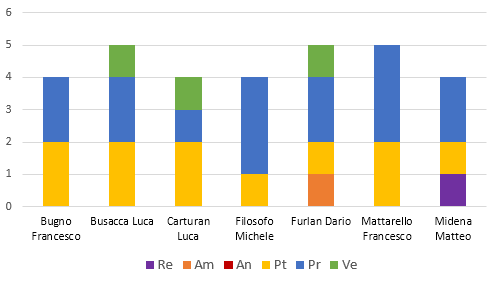
\includegraphics[scale=1.0]{immagini/5Sprint_oreLavoro.png}
  \caption{Suddivisione delle ore di lavoro - Sprint 5}
\end{figure}

\pagebreak
%%%%%%%%%%%%%%%%%%%%%%%%%%%%%%%%%%%%%%%%%%%%%%%%%%%%%%%%%%%%%%
In questo periodo i costi da affrontare per ogni ruolo sono i seguenti:

\begin{table}[H]
  \centering
  \renewcommand{\arraystretch}{1.8}
  \rowcolors{2}{green!100!black!40}{green!100!black!30}
  \begin{tabular}{c|c|c}
    \rowcolor[HTML]{125E28}
    \multicolumn{1}{c}{\color[HTML]{FFFFFF}\textbf{Ruolo}}
                    & \multicolumn{1}{c}{\color[HTML]{FFFFFF}\textbf{Ore}}
                    & \multicolumn{1}{c}{\color[HTML]{FFFFFF}\textbf{Costo (€)}}                   \\
    \hline
    Responsabile    & 1                                                          & 30,00           \\
    Amministratore  & 1                                                          & 20,00           \\
    Analista        & -                                                          & -               \\
    Progettista     & 11                                                         & 275,00          \\
    Programmatore   & 15                                                         & 225,00          \\
    Verificatore    & 3                                                          & 45,00           \\
    \textbf{Totale} & \textbf{31}                                                & \textbf{595,00}
  \end{tabular}
  \caption{Prospetto dei costi per ruolo - Sprint 5}
\end{table}

\begin{figure}[H]
  \centering
  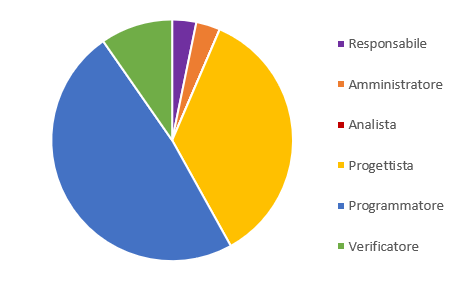
\includegraphics[scale=0.8]{immagini/5Sprint_oreRuolo.png}
  \caption{Ore per ruolo sul totale - Sprint 5}
\end{figure}

\begin{figure}[H]
  \centering
  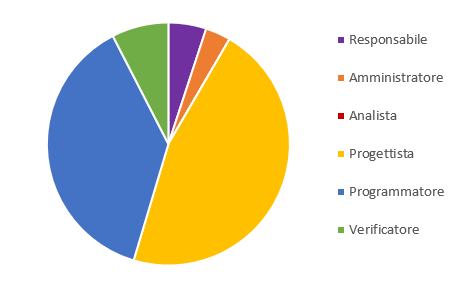
\includegraphics[scale=0.8]{immagini/5Sprint_costoRuolo.png}
  \caption{Costo per ruolo sul totale - Sprint 5}
\end{figure}
\pagebreak

%%%%%%%%%%%%%%%%%%%%%%%%%%%%%%%%%%%%%%%%%%%%%%%%%%%%%%%%%%%%%%

\paragraph{Sprint 6} \label{paragraph:preventivo_sprint6}
Nel sesto Sprint\glo{}, ciascun componente rivestirà i ruoli secondo la seguente suddivisione:

\begin{table}[H]
  \centering
  \renewcommand{\arraystretch}{1.8}
  \rowcolors{2}{green!100!black!40}{green!100!black!30}
  \begin{tabular}{c|c|c|c|c|c|c|c}
    \rowcolor[HTML]{125E28}
    \multicolumn{1}{c}{\color[HTML]{FFFFFF}\textbf{ Nominativo }}
                         & \multicolumn{1}{c}{\color[HTML]{FFFFFF}\textbf{ Re }}
                         & \multicolumn{1}{c}{\color[HTML]{FFFFFF}\textbf{ Am}}
                         & \multicolumn{1}{c}{\color[HTML]{FFFFFF}\textbf{ An }}
                         & \multicolumn{1}{c}{\color[HTML]{FFFFFF}\textbf{ Pt }}
                         & \multicolumn{1}{c}{\color[HTML]{FFFFFF}\textbf{ Pr }}
                         & \multicolumn{1}{c}{\color[HTML]{FFFFFF}\textbf{ Ve }}
                         & \multicolumn{1}{c}{\color[HTML]{FFFFFF}\textbf{ Ore totali }}                                                                                 \\
    \hline
    Bugno Francesco      & 1                                                             & -          & -          & 1          & 2           & -          & 4           \\
    Busacca Luca         & -                                                             & 2          & -          & 0          & 1           & 1          & 4           \\
    Carturan Luca        & -                                                             & -          & -          & 1          & 2           & 1          & 4           \\
    Filosofo Michele     & -                                                             & -          & -          & 1          & 2           & 1          & 4           \\
    Furlan Dario         & -                                                             & -          & -          & 2          & 1           & 1          & 4           \\
    Mattarello Francesco & -                                                             & -          & -          & 1          & 1           & 2          & 4           \\
    Midena Matteo        & -                                                             & -          & -          & 1          & 2           & 1          & 4           \\
    \textbf{Ore totali}  & \textbf{1}                                                    & \textbf{2} & \textbf{-} & \textbf{7} & \textbf{11} & \textbf{7} & \textbf{28}
  \end{tabular}
  \caption{Distribuzione delle ore durante il sesto Sprint}
\end{table}

I valori sono riassunti graficamente nel seguente grafico:

\begin{figure}[H]
  \centering
  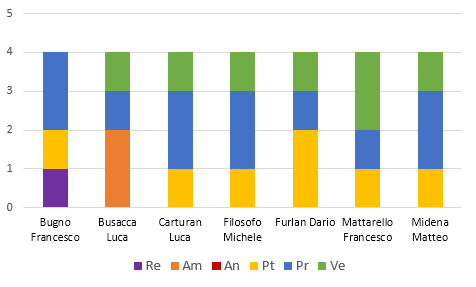
\includegraphics[scale=1.0]{immagini/6Sprint_oreLavoro.png}
  \caption{Suddivisione delle ore di lavoro - Sprint 6}
\end{figure}

\pagebreak
%%%%%%%%%%%%%%%%%%%%%%%%%%%%%%%%%%%%%%%%%%%%%%%%%%%%%%%%%%%%%%
In questo periodo i costi da affrontare per ogni ruolo sono i seguenti:

\begin{table}[H]
  \centering
  \renewcommand{\arraystretch}{1.8}
  \rowcolors{2}{green!100!black!40}{green!100!black!30}
  \begin{tabular}{c|c|c}
    \rowcolor[HTML]{125E28}
    \multicolumn{1}{c}{\color[HTML]{FFFFFF}\textbf{Ruolo}}
                    & \multicolumn{1}{c}{\color[HTML]{FFFFFF}\textbf{Ore}}
                    & \multicolumn{1}{c}{\color[HTML]{FFFFFF}\textbf{Costo (€)}}                   \\
    \hline
    Responsabile    & 1                                                          & 30,00           \\
    Amministratore  & 2                                                          & 40,00           \\
    Analista        & -                                                          & -               \\
    Progettista     & 7                                                          & 175,00          \\
    Programmatore   & 11                                                         & 165,00          \\
    Verificatore    & 7                                                          & 105,00          \\
    \textbf{Totale} & \textbf{28}                                                & \textbf{515,00}
  \end{tabular}
  \caption{Prospetto dei costi per ruolo - Sprint 6}
\end{table}

\begin{figure}[H]
  \centering
  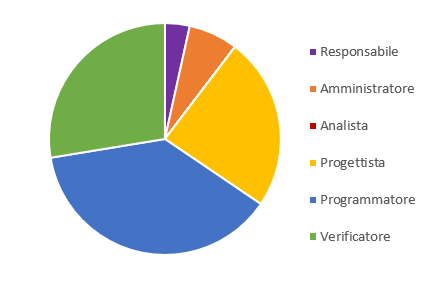
\includegraphics[scale=0.8]{immagini/6Sprint_oreRuolo.png}
  \caption{Ore per ruolo sul totale - Sprint 6}
\end{figure}

\begin{figure}[H]
  \centering
  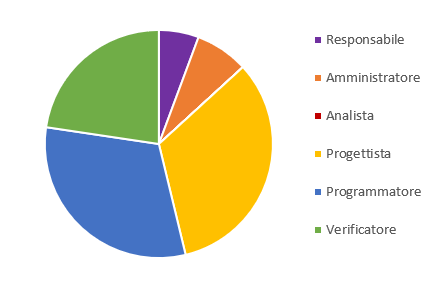
\includegraphics[scale=0.8]{immagini/6Sprint_costoRuolo.png}
  \caption{Costo per ruolo sul totale - Sprint 6}
\end{figure}
\pagebreak

%%%%%%%%%%%%%%%%%%%%%%%%%%%%%%%%%%%%%%%%%%%%%%%%%%%%%%%%%%%%%%

\subsubsection{Validazione e collaudo} \label{subsubsection:preventivo_validazione}
\paragraph{Sprint 7} \label{paragraph:preventivo_sprint7}
Nel settimo Sprint\glo{}, ciascun componente rivestirà i ruoli secondo la seguente suddivisione:

\begin{table}[H]
  \centering
  \renewcommand{\arraystretch}{1.8}
  \rowcolors{2}{green!100!black!40}{green!100!black!30}
  \begin{tabular}{c|c|c|c|c|c|c|c}
    \rowcolor[HTML]{125E28}
    \multicolumn{1}{c}{\color[HTML]{FFFFFF}\textbf{ Nominativo }}
                         & \multicolumn{1}{c}{\color[HTML]{FFFFFF}\textbf{ Re }}
                         & \multicolumn{1}{c}{\color[HTML]{FFFFFF}\textbf{ Am}}
                         & \multicolumn{1}{c}{\color[HTML]{FFFFFF}\textbf{ An }}
                         & \multicolumn{1}{c}{\color[HTML]{FFFFFF}\textbf{ Pt }}
                         & \multicolumn{1}{c}{\color[HTML]{FFFFFF}\textbf{ Pr }}
                         & \multicolumn{1}{c}{\color[HTML]{FFFFFF}\textbf{ Ve }}
                         & \multicolumn{1}{c}{\color[HTML]{FFFFFF}\textbf{ Ore totali }}                                                                                  \\
    \hline
    Bugno Francesco      & -                                                             & -          & -          & 2           & 2           & 2          & 6           \\
    Busacca Luca         & -                                                             & -          & -          & 2           & 3           & -          & 5           \\
    Carturan Luca        & -                                                             & -          & -          & 1           & 3           & 2          & 6           \\
    Filosofo Michele     & -                                                             & -          & -          & 2           & 2           & 1          & 5           \\
    Furlan Dario         & -                                                             & -          & -          & 2           & 3           & 1          & 6           \\
    Mattarello Francesco & 3                                                             & -          & -          & -           & 1           & 2          & 6           \\
    Midena Matteo        & -                                                             & 3          & -          & 1           & 2           & -          & 6           \\
    \textbf{Ore totali}  & \textbf{3}                                                    & \textbf{3} & \textbf{-} & \textbf{10} & \textbf{16} & \textbf{8} & \textbf{40}
  \end{tabular}
  \caption{Distribuzione delle ore durante il settimo Sprint}
\end{table}

I valori sono riassunti graficamente nel seguente grafico:

\begin{figure}[H]
  \centering
  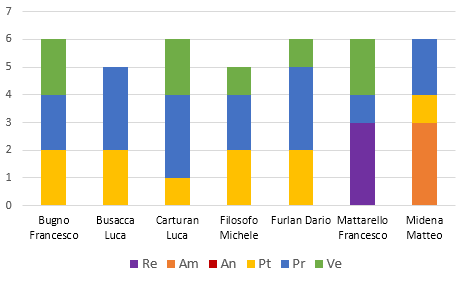
\includegraphics[scale=1.0]{immagini/7Sprint_oreLavoro.png}
  \caption{Suddivisione delle ore di lavoro - Sprint 7}
\end{figure}

\pagebreak
%%%%%%%%%%%%%%%%%%%%%%%%%%%%%%%%%%%%%%%%%%%%%%%%%%%%%%%%%%%%%%
In questo periodo i costi da affrontare per ogni ruolo sono i seguenti:

\begin{table}[H]
  \centering
  \renewcommand{\arraystretch}{1.8}
  \rowcolors{2}{green!100!black!40}{green!100!black!30}
  \begin{tabular}{c|c|c}
    \rowcolor[HTML]{125E28}
    \multicolumn{1}{c}{\color[HTML]{FFFFFF}\textbf{Ruolo}}
                    & \multicolumn{1}{c}{\color[HTML]{FFFFFF}\textbf{Ore}}
                    & \multicolumn{1}{c}{\color[HTML]{FFFFFF}\textbf{Costo (€)}}                   \\
    \hline
    Responsabile    & 3                                                          & 90,00           \\
    Amministratore  & 3                                                          & 60,00           \\
    Analista        & -                                                          & -               \\
    Progettista     & 10                                                         & 250,00          \\
    Programmatore   & 16                                                         & 240,00          \\
    Verificatore    & 8                                                          & 120,00          \\
    \textbf{Totale} & \textbf{40}                                                & \textbf{760,00}
  \end{tabular}
  \caption{Prospetto dei costi per ruolo - Sprint 7}
\end{table}

\begin{figure}[H]
  \centering
  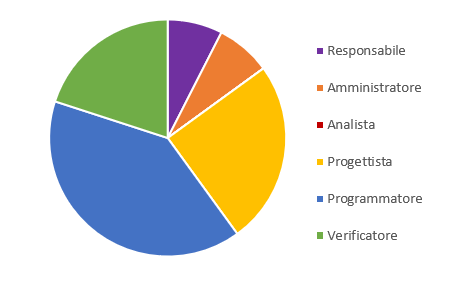
\includegraphics[scale=0.8]{immagini/7Sprint_oreRuolo.png}
  \caption{Ore per ruolo sul totale - Sprint 7}
\end{figure}

\begin{figure}[H]
  \centering
  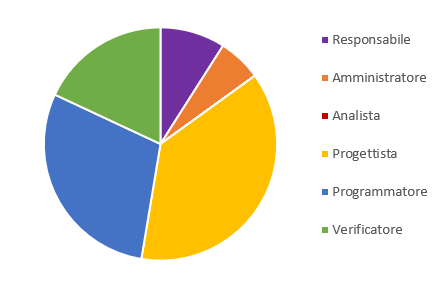
\includegraphics[scale=0.8]{immagini/7Sprint_costoRuolo.png}
  \caption{Costo per ruolo sul totale - Sprint 7}
\end{figure}
\pagebreak

%%%%%%%%%%%%%%%%%%%%%%%%%%%%%%%%%%%%%%%%%%%%%%%%%%%%%%%%%%%%%%
\subsection{Riepilogo Preventivo Iniziale} \label{subsection:preventivo_riepilogo}
In questa sezione viene presentato il riepilogo della suddivisione delle ore di lavoro ed il rispettivo costo preventivato inizialmente.

\begin{table}[H]
  \centering
  \renewcommand{\arraystretch}{1.8}
  \rowcolors{2}{green!100!black!40}{green!100!black!30}
  \begin{tabular}{c|c|c|c|c|c|c|c}
    \rowcolor[HTML]{125E28}
    \multicolumn{1}{c}{\color[HTML]{FFFFFF}\textbf{ Nominativo }}
                         & \multicolumn{1}{c}{\color[HTML]{FFFFFF}\textbf{ Re }}
                         & \multicolumn{1}{c}{\color[HTML]{FFFFFF}\textbf{ Am}}
                         & \multicolumn{1}{c}{\color[HTML]{FFFFFF}\textbf{ An }}
                         & \multicolumn{1}{c}{\color[HTML]{FFFFFF}\textbf{ Pt }}
                         & \multicolumn{1}{c}{\color[HTML]{FFFFFF}\textbf{ Pr }}
                         & \multicolumn{1}{c}{\color[HTML]{FFFFFF}\textbf{ Ve }}
                         & \multicolumn{1}{c}{\color[HTML]{FFFFFF}\textbf{ Ore totali }}                                                                                          \\
    \hline
    Bugno Francesco      & 11                                                            & 5           & 12           & 20           & 23           & 29           & 100          \\
    Busacca Luca         & 4                                                             & 17          & 10           & 20           & 25           & 24           & 100          \\
    Carturan Luca        & 12                                                            & 5           & 10           & 23           & 28           & 22           & 100          \\
    Filosofo Michele     & 6                                                             & 8           & 19           & 24           & 17           & 26           & 100          \\
    Furlan Dario         & 7                                                             & 10          & 19           & 24           & 15           & 25           & 100          \\
    Mattarello Francesco & 7                                                             & 18          & 12           & 23           & 16           & 24           & 100          \\
    Midena Matteo        & 8                                                             & 7           & 23           & 16           & 26           & 20           & 100          \\
    \textbf{Ore totali}  & \textbf{55}                                                   & \textbf{70} & \textbf{105} & \textbf{150} & \textbf{150} & \textbf{170} & \textbf{700}
  \end{tabular}
  \caption{Riepilogo della distribuzione delle ore di lavoro}
\end{table}

I valori sono riassunti graficamente nel seguente grafico:

\begin{figure}[H]
  \centering
  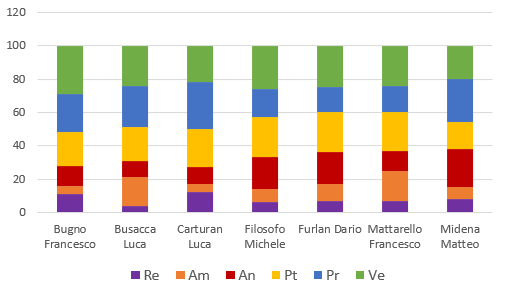
\includegraphics[scale=1.2]{immagini/ore_lavoro_riepilogo.png}
  \caption{Suddivisione delle ore di lavoro - Riepilogo}
\end{figure}

\pagebreak
%%%%%%%%%%%%%%%%%%%%%%%%%%%%%%%%%%%%%%%%%%%%%%%%%%%%%%%%%%%%%%
I costi da affrontare per ogni ruolo sono i seguenti:

\begin{table}[H]
  \centering
  \renewcommand{\arraystretch}{1.8}
  \rowcolors{2}{green!100!black!40}{green!100!black!30}
  \begin{tabular}{c|c|c}
    \rowcolor[HTML]{125E28}
    \multicolumn{1}{c}{\color[HTML]{FFFFFF}\textbf{Ruolo}}
                    & \multicolumn{1}{c}{\color[HTML]{FFFFFF}\textbf{Ore}}
                    & \multicolumn{1}{c}{\color[HTML]{FFFFFF}\textbf{Costo (€)}}                     \\
    \hline
    Responsabile    & 55                                                         & 1650,00           \\
    Amministratore  & 70                                                         & 1400,00           \\
    Analista        & 105                                                        & 2625,00           \\
    Progettista     & 150                                                        & 3750,00           \\
    Programmatore   & 150                                                        & 2250,00           \\
    Verificatore    & 170                                                        & 2550,00           \\
    \textbf{Totale} & \textbf{700}                                               & \textbf{14225,00}
  \end{tabular}
  \caption{Riepilogo del prospetto dei costi per ruolo}
\end{table}

\begin{figure}[H]
  \centering
  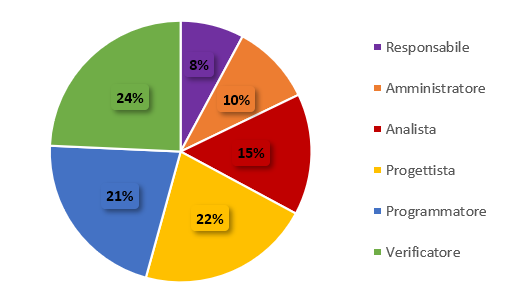
\includegraphics[scale=0.9]{immagini/ore_ruolo_riepilogo.png}
  \caption{Riepilogo delle ore per ruolo sul totale}
\end{figure}

\begin{figure}[H]
  \centering
  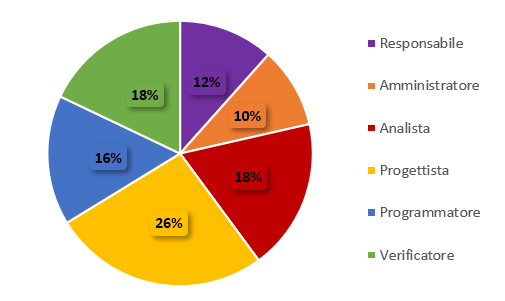
\includegraphics[scale=0.9]{immagini/costo_ruolo_riepilogo.png}
  \caption{Riepilogo del costo per ruolo sul totale}
\end{figure}

%%%%%%%%%%%%%%%%%%%%%%%%%%%%%%%%%%%%%%%%%%%%%%%%%%%%%%%%%%%%%%
